\section{Réduction d'espace d'état}
\label{sec:slicing}    

    % Program Slicing

    Le \emph{program slicing} \cite{Wei81}, est le calcul d'un sous-ensemble
    d'instructions (\emph{slice}) d'un programme qui affecte les valeurs d'un
    sous-ensemble de ses variables à un certain moment de son exécution. Ce
    sous-ensemble d'instructions est tel qu'il possède un comportement
    équivalent au programme originial vis-à-vis de la valuation du sous-ensemble
    de variables du programme considéré.

    Un \emph{slice} est calculé vis-à-vis d'un critère de \emph{slice}. Celui-ci
    détermine le sous-ensemble des variables du programme ainsi que l'instant
    d'exécution pris en compte. $\mathcal{C}$ est un critère de \emph{slice} tel
    que $\mathcal{C} = \langle l, V \rangle$ avec $l \in \mathcal{L}$ et $V
    \subseteq \mathcal{V}$. Les figures \ref{fig:slice1} et \ref{fig:slice2}
    donne les \emph{slices} du programme \texttt{fibcall-O2.elf} (cf. figure
    \ref{fig:dump}) respectivement pour le critère $\mathcal{C} = \langle 302c,
    \{ r10 \} \rangle$ et le critère $\mathcal{C} = \langle 3030, \{ ctr \}
    \rangle$. $R$ est l'ensemble des variables -- ou registres ici --
    explicitement ou implicitement manipulés qui font l'objet de dépendances de
    données entre les différents blocs de base du CFG. Autrement dit, ce sont
    les variables qui sont à conserver dans l'espace d'état du système pour en
    réaliser une analyse précise et efficace vis-à-vis de leurs valuations
    possibles.

    \begin{figure}[ht]
      \centering
      \begin{subfigure}{.45\textwidth}
        \centering
        \captionsetup{justification=centering}
        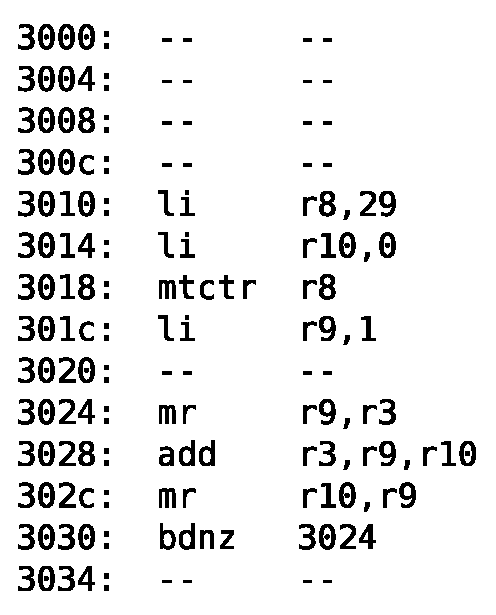
\includegraphics[scale=0.45]{img/slice1.eps}
        \caption{\emph{slice} pour le critère $\mathcal{C} = \langle 302c, \{ r10 \} \rangle$ \\
          $R = \{r3, r8, r9, r10, ctr\}$}
        \label{fig:slice1}
      \end{subfigure}
      \begin{subfigure}{.45\textwidth}
        \centering
        \captionsetup{justification=centering}
        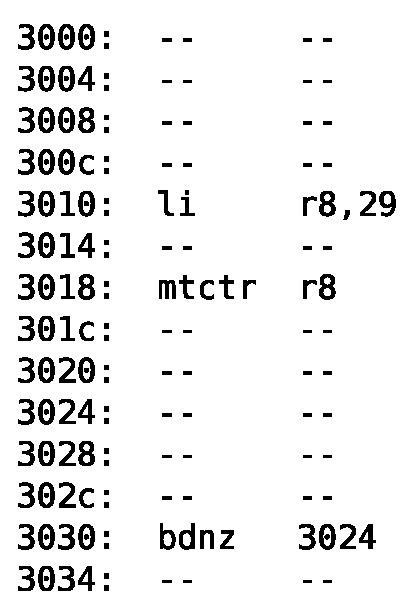
\includegraphics[scale=0.45]{img/slice2.eps}
        \caption{\emph{slice} pour le critère $\mathcal{C} = \langle 3030, \{ ctr \} \rangle$ \\
        $R = \{ctr\}$}
        \label{fig:slice2}
      \end{subfigure}
      \caption{Exemple de \emph{program slicing} d'un fichier binaire exécutable}
    \end{figure}

    %% Quand le \emph{slicing} s'applique à une seule procédure monolithique on
    %% parle de \emph{slicing} intraprocédural. En revanche lorsque le
    %% \emph{slicing} s'applique à un programme entier, au delà des frontières
    %% d'une procédure, on parle de \emph{slicing} interprocedural.
  
    % Intérêt du Program Slicing des CFG pour la vérification de modèle.

    Pour pallier au problème de l'explosion de l'espace d'état inhérent à la
    vérification des modèles il est nécessaire de réduire au maximum la quantité
    d'informations définisant l'état du système. Une utilisation spécifique du
    \emph{program slicing} permet de ne conserver dans l'espace d'état
    du système uniquement les informations définissant l'état des variables --
    registre ou contenu de la pile -- dont la valuation influt directement sur
    le flot de contrôle.

    Il n'est, en effet, pas nécessaire de conserver dans l'espace d'état du
    système les valuations de toutes les variables qui n'agissent pas
    directement sur le flot de contrôle puisqu'elles n'influent pas sur le temps
    d'exécution. Le \emph{slice} donné en figure \ref{fig:slice2} contient
    l'ensemble des instructions du programme \texttt{fibcall-O2.elf} qui agissent
    directement sur le flot de contrôle et manipulent des variables explicitement
    ou implicitement. Il est donc nécessaire de conserver dans l'espace d'état
    du système uniquement la valuation d'un seul registre ($R = \{ ctr$ \}) au
    lieu des 7 registres originaux ($R = \{r1, r3, r8, r9, r10, lr, ctr\}$,
    cf. figure \ref{fig:dump}).
     
    \vspace{1em}
  
    % Program Slicing à base de graphes

    Il existe différentes approches permettant de calculer un \emph{slice}
    \cite{Tip95}.  Cependant, seule la sous catégorie des approches basées sur
    la manipulation de graphes permet de calculer un \emph{slice} pour les
    fichiers binaires exécutables.
    
    Nous nous basons sur une approche permettant de calculer des \emph{slices}
    précis pour les programmes composés de plusieurs procédures (\emph{program
      slicing} interprocédural) \cite{KJL03}.
    
    %% L'algorithme de \emph{slicing} implémenté s'appuie sur la méthode évoquée
    %% ci-après -- cf. \cite{CF97}. Les dépendances de données du programme y sont
    %% représentées par l'arbre post-dominateur et par des chaines de
    %% \emph{use-definition}. Ces chaines relient chaque utilisation d'une
    %% variable aux définitions qui peuvent l'affecter.

    %% Les dépendances de contrôle du programme sont manipulés à travers un graphe
    %% de dépendance de contrôle. Un graphe de dépendance de contrôle est un graphe
    %% où les arcs signifient un lien de dépendance entre la valuation du n{\oe}ud
    %% origine et l'exécution du n{\oe}ud cible.
    
